% %% ========================================
\section{Proposed Solution}\label{sec:solution}

As shown in Fig.~\ref{fig:overall}, PushAround first constructs a
W-Clearance Connectivity Graph in Sec.~\ref{subsec:wccg} to capture
workspace connectivity and blocking gaps. Gap ranking in
Sec.~\ref{subsec:gap} selects obstacle-clearing actions, while mode
generation and evaluation in Sec.~\ref{subsec:push} ensure physically
feasible collaborative pushes. These components are integrated into the
simulation-in-the-loop hybrid search in Sec.~\ref{subsec:simloop}.
Sec.~\ref{subsec:overall} summarizes the overall online execution.





% %% ========================================
%==============================================
\subsection{W--Clearance Connectivity Graph}\label{subsec:wccg}

The feasibility of routing the vehicle reduces to whether a~$W$-width corridor
connects~$\mathbf{x}_\texttt{V}^{\texttt{S}}$ and~$\mathbf{x}_\texttt{V}^{\texttt{G}}$.
A W--clearance connectivity graph (WCCG) is introduced here to encode obstacle
adjacencies under clearance~$W$ and enable fast connectivity queries.
\change{Conventional clearance checks either rasterize the workspace into an
inflated occupancy grid or query sampling-based roadmaps, and must therefore fix
a resolution and re-query the map whenever an obstacle
moves~\cite{karaman2011samplingbasedalgorithmsoptimalmotion}.
Built directly from obstacle geometry, the WCCG introduces no grid-resolution parameter in the repeated connectivity queries used during planning.}

%------------------------------
\begin{figure}[t!]
  \centering
  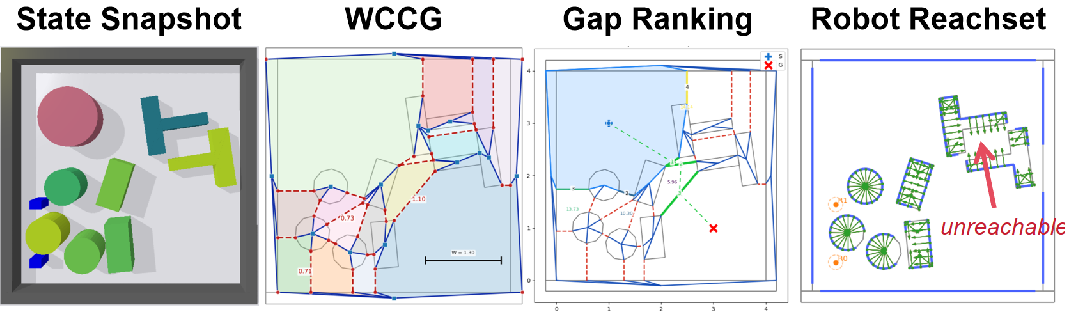
\includegraphics[width=0.9\linewidth]{figures/PIHS_top.pdf}
  \vspace{-2mm}
  \caption{\change{Core components of the physics-informed hybrid search: WCCG
  construction, gap ranking, mode generation, and physics validation.}}
  \label{fig:pihs_overview}
  \vspace{-4mm}
\end{figure}
%------------------------------

\subsubsection{Graph Construction}
The WCCG is built by decomposing all clearance-relevant obstacle and workspace
boundaries into convex components or segments.
From each component~$C$,
a centroid node~$v_c$ is created. When two components~$C_u$ and~$C_v$
have closest points~$p_u\in C_u$ and~$p_v\in C_v$ with distance less than~$W$,
bridge nodes are added at~$p_u$ and~$p_v$. These bridge nodes are
connected by a bridge--bridge edge, annotated with the gap width
$w_{uv}\triangleq\|p_u-p_v\|$, and further linked back to their centroids with
centroid--bridge edges. Narrow passages with~$w_{uv}<W$ are marked
as potential bottlenecks. The resulting graph is given by:
\begin{equation}\label{eq:wccg}
\mathcal{G}_W\triangleq(\mathcal{V},\; \mathcal{E}_c\cup\mathcal{E}_b),
\end{equation}
where~$\mathcal{V}$ are centroid and bridge nodes;
$\mathcal{E}_c$ contains centroid--bridge edges; and~$\mathcal{E}_b$ for
bridge--bridge edges with widths~$w_{uv}$.

\subsubsection{Connectivity Criterion}\label{subsubsec:bugplanner}
Once~$\mathcal{G}_W$ has been constructed, connectivity queries can be
performed without explicitly computing a geometric path. Let
$\textsf{Face}(\mathcal{G}_W)$ denote the set of connected planar faces induced
by the embedded WCCG, i.e., the maximal regions separated by obstacle
components and WCCG bottleneck edges. The criterion for~\eqref{eq:wclear}
is given by
\begin{equation}\label{eq:wccg_criterion}
\big(\mathbf{x}_\texttt{V}^{\texttt{S}},\mathbf{x}_\texttt{V}^{\texttt{G}}\in
\mathcal{F}_W(t)\big)
\wedge
\big( \exists F\in\textsf{Face}(\mathcal{G}_W):
{\mathbf{x}_\texttt{V}^{\texttt{S}},\mathbf{x}_\texttt{V}^{\texttt{G}}}\in F \big),
\end{equation}
\change{where the faces follow the standard configuration-space inflation
interpretation: expanding obstacles by a disk of radius $W/2$ turns gaps
narrower than $W$ into overlapping barriers, and non-convex obstacles are
handled through clearance-relevant decomposition, after which WCCG records the
separating bottlenecks.} The consistency between WCCG connectivity and continuous and
rasterized configuration-space references is further evaluated numerically
in Sec.~\ref{subsec:wccg-validation}.
A frontier-tracing procedure, similar to the
BugPlanner~\cite{McGuireCroonTuyls2019}, is then used to extract a skeleton
$\Sigma$ as an ordered sequence of centroid and bridge nodes. Starting from
$\mathbf{x}_\texttt{V}^{\texttt{S}}$, it casts a ray toward
$\mathbf{x}_\texttt{V}^{\texttt{G}}$ and follows the encountered frontier loop
until either a valid exit is found or a blocking cycle is returned.








%% \begin{algorithm}[t!]
%% \small
%% \caption{BugPlanner for~$W$-width connectivity (skeleton witness)}
%% \label{alg:bugplanner}
%% \DontPrintSemicolon
%% \SetKwInOut{Input}{In}\SetKwInOut{Output}{Out}
%% \Input{$\mathbf{s}^{\texttt{S}}$,~$\mathbf{s}^{\texttt{G}}$, WCCG}
%% \Output{if connected: skeleton~$\Sigma$; else: frontier loop~$\mathcal{L}$}
%%~$P\leftarrow\mathbf{s}^{\texttt{S}}$,~$\Sigma\leftarrow[\ ]$\;
%% \While{true}{
%%   \If{segment~$P\mathbf{s}^{\texttt{G}}$ hits no edge}{\Return~$\Sigma \cup \{\texttt{straight}(P,\mathbf{s}^{\texttt{G}})\}$}
%%   Build loop~$\mathcal{L}$ by angle-follow from the hit edge; append traversed edges to~$\Sigma$\;
%%   \If{$\mathrm{parity}(\mathcal{L},\,\mathbf{s}^{\texttt{S}}\mathbf{s}^{\texttt{G}})$ is odd}{\Return~$(\emptyset,\mathcal{L})$}
%%   Choose exit~$e$ on~$\mathcal{L}$ (outward normal~$\to\,\mathbf{s}^{\texttt{G}}$); append arc to~$\Sigma$;~$P\leftarrow e$ (tiny bias)\;
%% }
%% \end{algorithm}

% %% ========================================
%==============================================
\subsection{Ranking of Frontier Gaps}\label{subsec:gap}

When the condition in~\eqref{eq:wccg_criterion} fails, the vehicle cannot
reach~$\mathbf{x}_\texttt{V}^{\texttt{G}}$ from
$\mathbf{x}_\texttt{V}^{\texttt{S}}$ through a~$W$--clear path
$\mathcal{P}^W_\texttt{V}$.
In this case, the planner must prioritize
\emph{blocking gaps} on the reachable frontier of~$\mathcal{G}_W$
according to their predicted downstream cost, and feed the ranked list to the
hybrid search as local clearance targets.

\subsubsection{Frontier Extraction and Candidate Gaps}
A BugPlanner query on~$\mathcal{G}_W$ above
either confirms connectivity or returns a counter--clockwise frontier loop
$\mathcal{L}$ that separates the two endpoints. The bridge--bridge edges on
$\mathcal{L}$ define the first--hop candidate set
$\Gamma_\mathcal{L}\triangleq\{g_1,\cdots,g_K\}$,
where each gap~$g_k$ is represented by its two closest boundary points, its
width~$w_{g_k}<W$, and the adjacent obstacles that can potentially be moved.
These candidates are then ranked by predicted downstream cost and passed to the
hybrid search as local clearance targets.

\subsubsection{Evaluation for Immediate Cost}
Each candidate~$g\in\Gamma_\mathcal{L}$ is evaluated by combining the
cost for the robots to reach the gap and the effort required to widen it.
Let~$\mathbf{s}_{\mathcal{R}}$ be the current robot positions,
and~$\mathbf{o}_g$ as the outside insertion point of gap~$g$. The
resulting one--hop cost is given by:
\begin{equation}\label{eq:step_cost}
\mathsf{C}\big(g \mid \mathcal{L}, \mathbf{s}_{\mathcal{R}}\big)
=\lambda_\texttt{t}\,\mathsf{C}_\texttt{t}\!\left(\mathbf{s}_{\mathcal{R}},\mathbf{o}_g\right)
+\lambda_\texttt{p}\,\big( \mathsf{C}_\texttt{dp}(g) + \mathsf{C}_\texttt{rp}(g)\big)
\end{equation}
where~$\lambda_\texttt{t},\lambda_\texttt{p}>0$ weight transition and pushing costs, respectively; $\mathsf{C}_\texttt{t}$, $\mathsf{C}_\texttt{dp}$, and $\mathsf{C}_\texttt{rp}$ denote transition, direct-pushing, and recursive-pushing costs.

%------------------------------
\begin{figure}[t!]
  \centering
  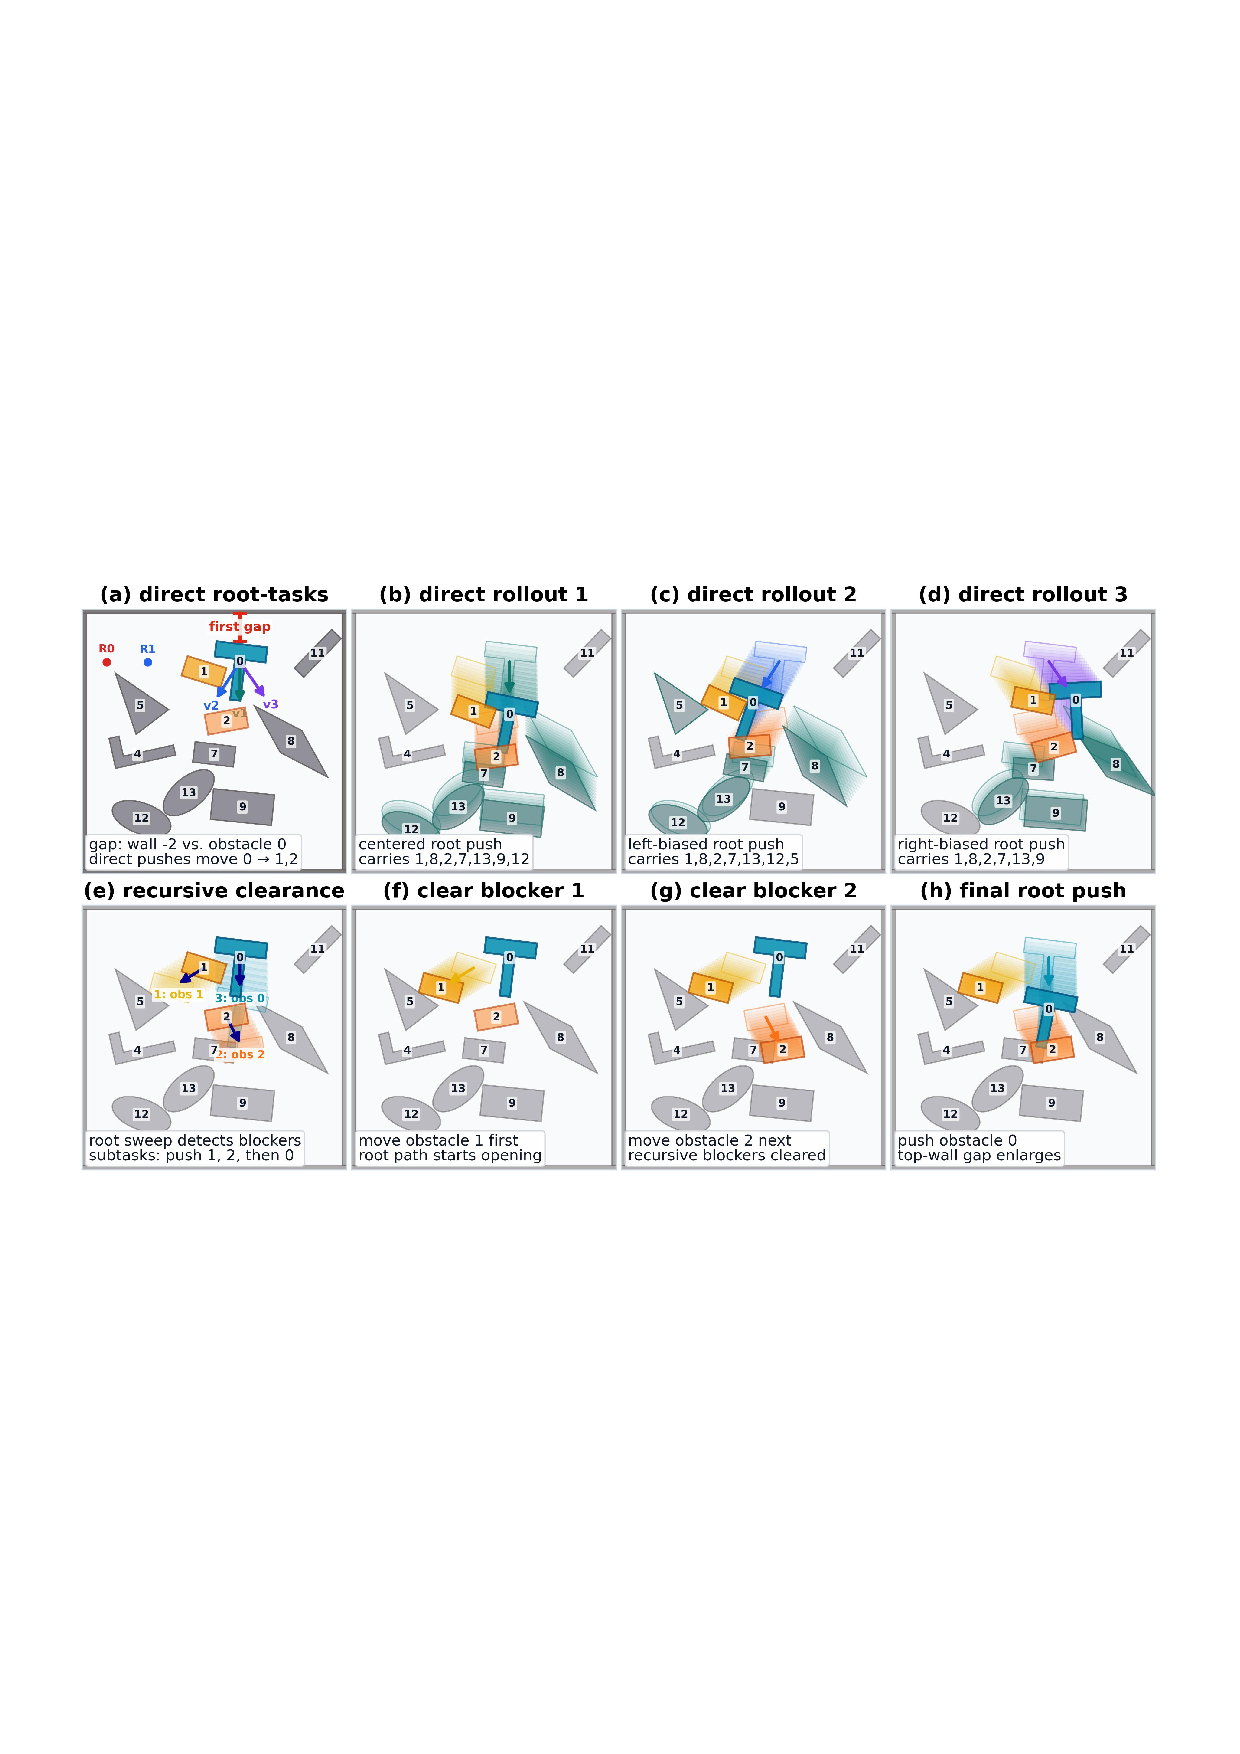
\includegraphics[width=0.82\linewidth]{figures/direct_recursive_push.pdf}
  \vspace{-0.1in}
  \caption{\change{
  \textbf{Direct} pushing moves a gap-side blocker along a gap-opening direction,
  whereas \textbf{recursive} pushing first clears movable blockers in the swept
  region and then returns to the root gap-opening task.}}
  \label{fig:direct_recursive_push}
  \vspace{-4mm}
\end{figure}
%------------------------------

\subsubsection{Long-term Cost w.r.t. Goal}
Furthermore, to prioritize gaps closer to the goal, a heuristic is added to the evaluation,
i.e.,
$h(g)=\eta\,\big\|\mathbf{o}(g)-\mathbf{x}_\texttt{V}^{\texttt{G}}\big\|$,
with the scaling constant~$\eta>0$.
Lastly, a short A$^\star$-style presearch is adopted to cross
each candidate gap, recompute the next frontier, and continue for a limited
width and depth. The \emph{cost-to-connect} is predicted by:
\begin{equation}\label{eq:pred_cost}
\widehat{\mathsf{Cost}}(g)\triangleq
\mathsf{C}\!\big(g \mid \mathcal{L},\mathbf{s}_{\mathcal{R}}\big)
+\!\!\!\sum_{g'\in\Pi^\star(g)}\!\!\!\big{\{}\mathsf{C}(g' \mid \cdot)+h(g')\big{\}},
\end{equation}
where~$\Pi^\star(g)$ is the sequence of subsequent gaps discovered after virtually crossing~$g$. Consequently, the final output of this module is the ranked list of candidate gaps, i.e.,
$\textsf{Rank}\big(\Gamma_\mathcal{L}\big)
\triangleq \textbf{argsort}_{g\in\Gamma_\mathcal{L}}\widehat{\mathsf{Cost}}(g)$,
in ascending predicted cost. This
ordered set is passed to the hybrid search module, such that only the
promising gaps are expanded first.



% %% ========================================
%==============================================
\subsection{Pushing Mode Generation and Evaluation}\label{subsec:push}
For a selected frontier gap~$g$, this subsection constructs a set of candidate
pushing strategies
$\Xi_g \triangleq \{(\Omega_m,\mathbf{v},\boldsymbol{\xi})\}$,
where~$\mathbf{v} \triangleq (v_x,v_y,\omega)\in\mathbb{R}^3$ is a
short-horizon pushing direction for the movable obstacle~$\Omega_m$ induced by~$g$, and
$\boldsymbol{\xi}\triangleq(\mathbf{c}_m,\mathbf{u})$ is the associated pushing
mode in~\eqref{eq:transition}.
\change{The wrench feasibility encoded in~$\boldsymbol{\xi}$ acts as a screening
condition rather than a force setpoint: it certifies that the chosen contact
configuration can realize the required object motion within the robots'
actuation limits, after which the candidate is passed to the physics rollout for
validation.}



%==============================================
\subsubsection{Direct and Recursive Pushing Tasks}
For \emph{direct push}, let~$\Omega_m$ denote one of the two movable obstacles adjacent to~$g$. For
each such obstacle, a small set of candidate body velocities
$\{\mathbf{v}_m^k\}_{k=1}^{K_m}$ is sampled with a bias toward enlarging the
gap~$g$, while a few angular components are included to account for local
geometry. If the swept region of a direct push intersects movable blockers,
\emph{recursive push} tasks are required instead: for each out-layer
blocker~$\Omega_m$, the nominal direction moves it away from both the swept
region and the reference gap sequence~$\Pi^\star(g)$. Recursion therefore
creates a bounded dependency chain which prioritizes the final
blocker~$\Omega_m$, as shown in Fig.~\ref{fig:direct_recursive_push}.






%==============================================
% \subsubsection{Pushing Mode Generation}
% For each sampled direction~$\mathbf{v}_m^k$ and obstacle~$\Omega_m$, the
% quality of a candidate mode is measured in the body frame. Let
% $\mathbf{v}_m^{k,\mathrm{B}} \in \mathbb{R}^3$ denote~$\mathbf{v}_m^k$
% expressed in the body frame of~$\Omega_m$. For a mode~$\boldsymbol{\xi}$,
% define the primary and multi-directional feasibility losses by:
% \begin{equation}\label{eq:mode-feasibility}
% \begin{aligned}
%   \mathrm{J}_{\texttt{F}}^m
%   (\boldsymbol{\xi},\mathbf{v}_m^{k,\mathrm{B}})
%   &\triangleq
%   \underset{\mathbf{q}_{m,\boldsymbol{\xi}} \in
%   \mathrm{Q}_{m,\boldsymbol{\xi}}}{\textbf{min}}
%   \left\|
%   \mathbf{q}_{m,\boldsymbol{\xi}} +
%   Q_\mu^m(\mathbf{v}_m^{k,\mathrm{B}})
%   \right\|_1,\\
%   \mathrm{J}_{\texttt{MF}}^m
%   (\boldsymbol{\xi},\mathbf{v}_m^{k,\mathrm{B}})
%   &\triangleq
%   \sum_{\mathbf{v}_d \in \mathcal{D}} w_d \cdot
%   \mathrm{J}_{\texttt{F}}^m(\boldsymbol{\xi},\mathbf{v}_d);
% \end{aligned}
% \end{equation}
% where~$\mathbf{q}_{m,\boldsymbol{\xi}} \in \mathbb{R}^3$ is the generalized
% body wrench induced by mode~$\boldsymbol{\xi}$;
% $\mathrm{Q}_{m,\boldsymbol{\xi}} \subseteq \mathbb{R}^3$ is the corresponding
% set of admissible body wrenches under the contact and friction constraints;
% $Q_\mu^m(\mathbf{v}_m^{k,\mathrm{B}}) \in \mathbb{R}^3$ denotes the
% quasi-static friction wrench of~$\Omega_m$ at direction~$\mathbf{v}_m^{k,\mathrm{B}}$;
% $\mathcal{D} \subset \mathbb{R}^3$ is a finite
% set of basis velocities containing the desired direction;
% and~$w_d > 0$ is the
% weight associated with~$\mathbf{v}_d \in \mathcal{D}$. Thus,
% small~$\mathrm{J}_{\texttt{F}}^m(\boldsymbol{\xi},\mathbf{v}_m^{k,\mathrm{B}})$ is
% necessary for force feasibility, while small
% $\mathrm{J}_{\texttt{MF}}^m$ indicates a robust mode.
% Accordingly, the associated mode
% $\boldsymbol{\xi}_m^k \triangleq (\mathbf{c}_m^k,\mathbf{u}_m^k)$ is generated
% by sparse optimization over the reachable part of~$\partial\Omega_m$. The
% reachable boundary is discretized into candidate contacts, and a sparse linear
% program (LP) is solved to minimize
% $\mathrm{J}_{\texttt{MF}}^m(\boldsymbol{\xi},\mathbf{v}_m^{k,\mathrm{B}})$
% under the local friction and wrench constraints.
% Detailed derivations are omitted here for brevity,
% and referred to~\cite{tang2024collaborative,tang2025pushingbots}.
% The resulting nonzero contacts provide~$\mathbf{c}_m^k$, and the corresponding forces
% yield~$\mathbf{u}_m^k$. Only the best few
% pairs~$(\mathbf{v}_m^k,\boldsymbol{\xi}_m^k)$ are retained and collected
% into~$\Xi_g$.

\subsubsection{Pushing Mode Generation}
At a search state~$\mathbf{s}$, a pushing mode is generated for each candidate
direction~$\mathbf{v}_m^k$ and obstacle~$\Omega_m$. In this subsubsection,
contact tuples, object velocities, forces, and wrenches are expressed in the
body frame of~$\Omega_m$. For a contact tuple~$\mathbf{c}$, its
multi-directional force feasibility is:
\begin{equation}\label{eq:mode-feasibility}
\mathrm{J}_{\texttt{MF}}^m(\mathbf{c},\mathbf{v}_m^k)
\triangleq
\sum_{\mathbf{v}_d\in\mathcal{D}_m^k} w_d
\underset{\mathbf{u}\in{U}_m(\mathbf{c})}{\textbf{min}}
\|
\mathbf{q}_m(\mathbf{c},\mathbf{u})
+\mathbf{q}_m^\mu(\mathbf{v}_d)
\| ,
\end{equation}
where~$\|\cdot\|$ is a weighted $\ell_1$ wrench norm, the finite set
$\mathcal{D}_m^k$ perturbs~$\mathbf{v}_m^k$, and
$\mathbf{q}_m^\mu(\mathbf{v}_d)$ is the quasi-static friction wrench; the inner
minimization is a small LP over the admissible forces ${U}_m(\mathbf{c})$.
A state- and direction-dependent contact set
$\mathcal{A}_m^k(\mathbf{s})\subset\partial\Omega_m$ is drawn from the
robot-reachable boundary of~$\Omega_m$ by velocity--force compatibility
filtering (Fig.~\ref{fig:mode_generation}), keeping a contact only if its
robots reach collision-free pre-contact poses. Starting from cached layouts or
random initializations, the tuple is refined by sequential greedy replacement:
at the $\ell$-th step, $\mathbf{c}_{r,c}^{\ell}$ replaces the $r$-th contact
with $c$, and the best replacement is:
\begin{equation}
c^\star
=
\underset{c\in\mathcal{A}_m^k(\mathbf{s})}{\textbf{argmin}}\;
\mathrm{J}_{\texttt{MF}}^m
\bigl(\mathbf{c}_{r,c}^{\ell},\mathbf{v}_m^k\bigr),
\label{eq:greedy_mode_update}
\end{equation}
swept over contact slots until $\mathrm{J}_{\texttt{MF}}^m$ no longer
decreases; a bounded backtracking variant removes the robot-order sensitivity
of this replacement. If no full-team assignment exists for a task, e.g., on
small faces or under the pairwise pusher-clearance constraint, one robot is
released for that single push (charged a penalty when ranking modes, so
full-team modes are preferred) and the full team is available again afterwards.
The best tuple over initializations gives
$\mathbf{c}_m^{k,\star}$, from which $\mathbf{u}_m^k$ follows from the inner
minimization in~\eqref{eq:mode-feasibility}, yielding
$\boldsymbol{\xi}_m^k=(\mathbf{c}_m^{k,\star},\mathbf{u}_m^k)$; each mode is
cached as a warm start. The best few admissible pairs are kept for gap~$g$ and
passed to simulation; $\mathbf{u}_m^k$ certifies wrench feasibility while
hardware tracks the contact geometry from pose/velocity commands.

% The best refined mode over all initializations is denoted by
% $\boldsymbol{\xi}_m^k=(\mathbf{c}_m^k,\mathbf{u}_m^k)$.
% It is admitted only if its rollout is validated in simulation.
% Accepted modes are stored in a persistent \textsc{mode-cache},
% indexed by discretized shape, mass, available robot force, and pushing direction,
% and reused as warm starts.
%------------------------------
\begin{figure}[t!]
  \centering
  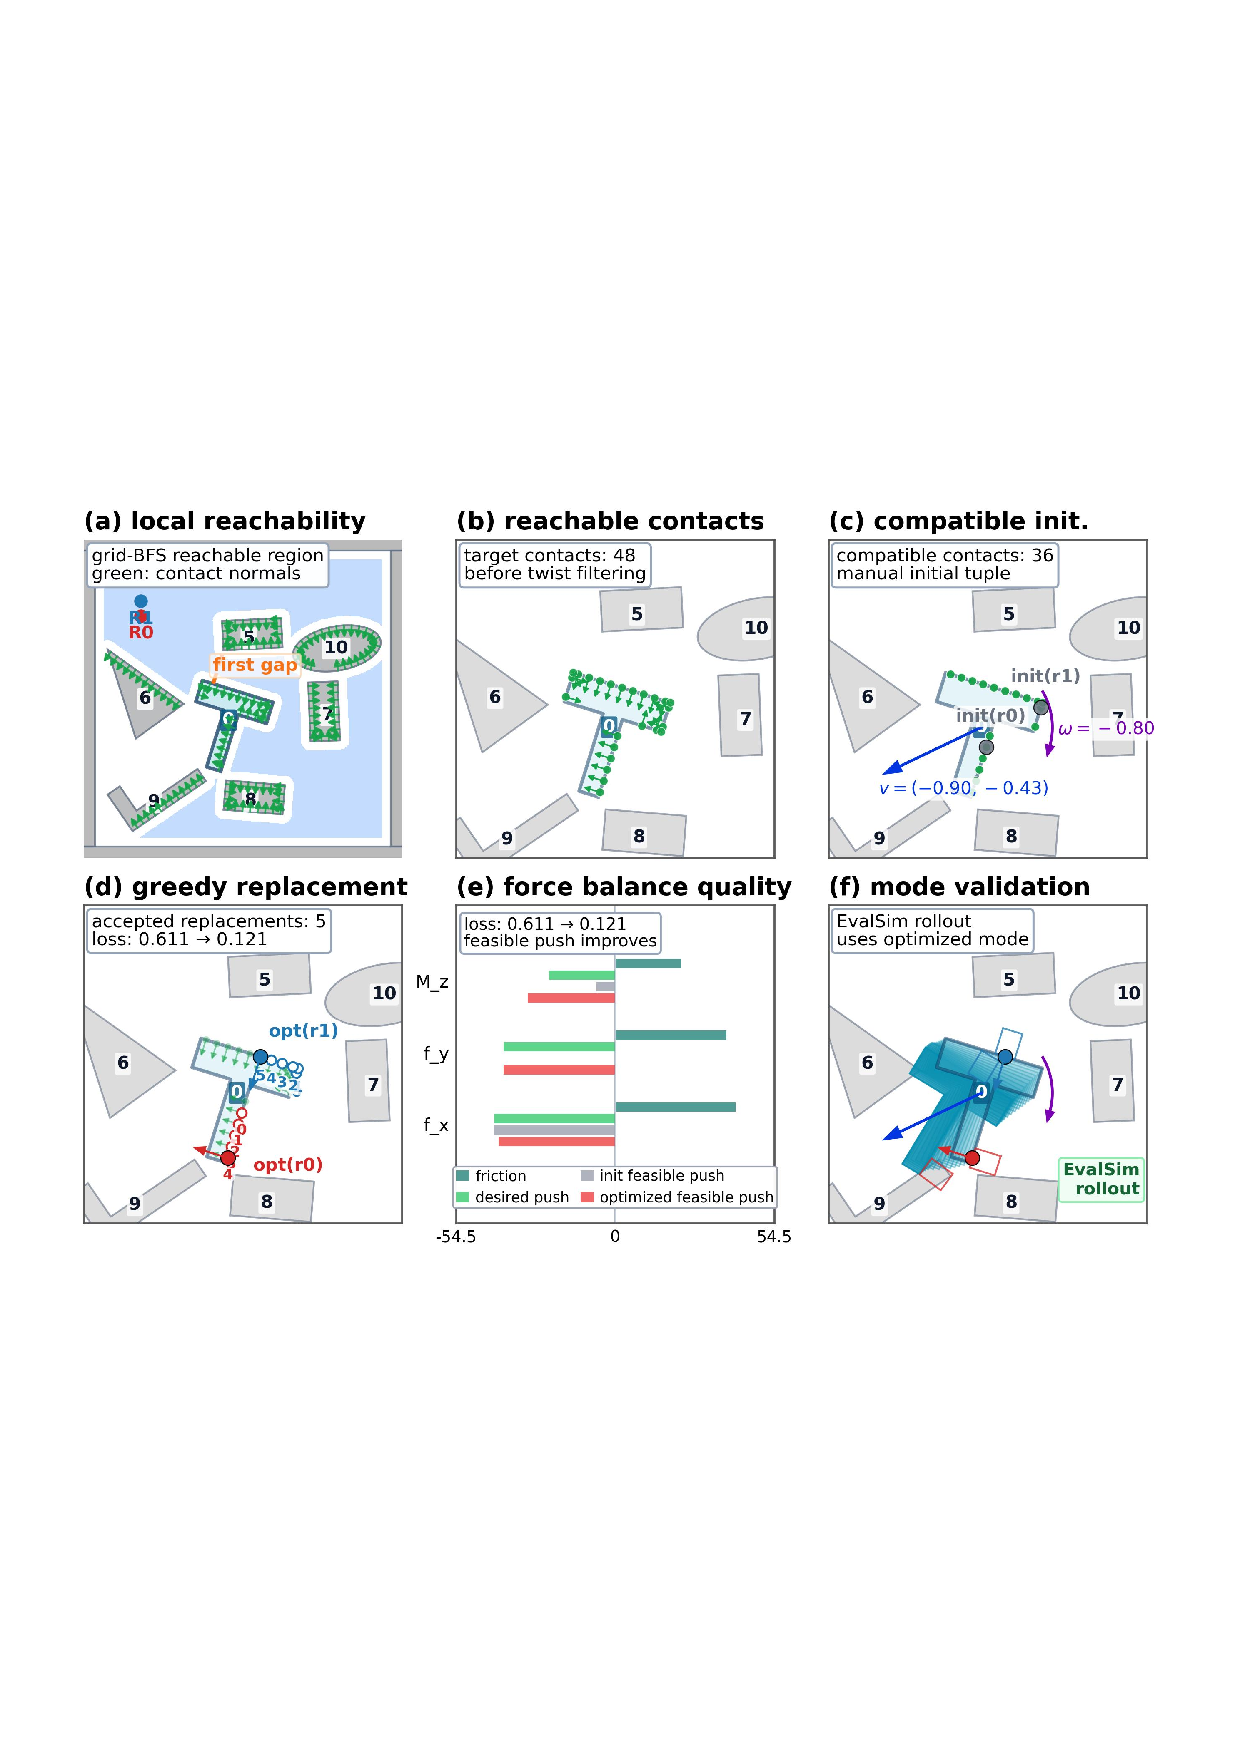
\includegraphics[width=0.8\linewidth]{figures/mode_generation.pdf}
  \vspace{-4mm}
  \caption{\change{
Reachable contacts are filtered by the
  desired object twist, assigned to robots, refined by local replacement,
  and finally validated by simulation.}}
    \label{fig:mode_generation}
   \vspace{-4mm}
\end{figure}
%------------------------------
%==============================================
\subsubsection{Pushing Strategy Evaluation}

For a current state~$\mathbf{s}$ and a candidate strategy
$(\Omega_m,\mathbf{v},\boldsymbol{\xi})\in\Xi_g$, a short-horizon rollout
evaluates the transition in~\eqref{eq:transition} under the selected mode.
As shown in Fig.~\ref{fig:mode_generation}, a strategy is accepted only if
the robots reach the pre-contact poses, maintain stable contact, and induce
obstacle motion above threshold. The simulation returns:
\begin{equation}
    (\mathbf{s}',\,\delta_{\texttt{T}},\,\delta_{\texttt{J}})
    \triangleq
    \mathsf{EvalSim}
    \big(
    \mathbf{s},(\Omega_m,\mathbf{v},\boldsymbol{\xi})
    \big),
    \label{eq:sim}
\end{equation}
where~$\mathbf{s}'$ is the successor state capturing the resulting robot and
object configurations; $\delta_{\texttt{T}}>0$ is the time cost; and
$\delta_{\texttt{J}}$ is the control effort. 
\change{
The rollout jointly simulates
all robots and movable bodies, thereby capturing contact-induced object
interactions.}
For efficiency, the pushing rollout may be bypassed when the mode has been
validated before and the swept region of~$\Omega_m$ is collision-free.
%------------------------------
\begin{figure}[t!]
  \centering
  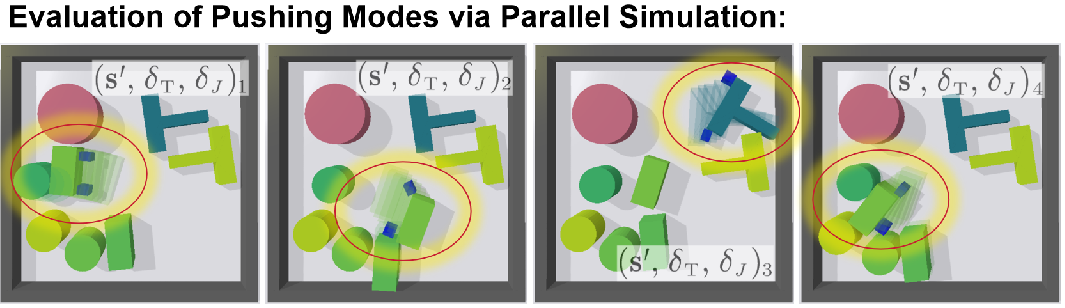
\includegraphics[width=0.8\linewidth]{figures/PIHS_bottom.pdf}
  \vspace{-2mm}
  \caption{\change{Sampled push tasks are evaluated via parallel simulation,
  producing updated states for search expansion.}}
    \label{fig:PIHS}
   \vspace{-4mm}
\end{figure}
%------------------------------

% %% ========================================
%==============================================
\subsection{Physics-Informed Hybrid Search}\label{subsec:simloop}

As shown in Fig.~\ref{fig:PIHS}, the physics-informed hybrid search~(PIHS)
couples WCCG-guided gap sequencing, recursive push-task generation,
contact-mode optimization, and short-horizon physics rollout. A search node is a
simulated system snapshot, and a push task labels each tree edge. Auxiliary
records, including parent pointer, incoming task, gap-sequencing cache,
accumulated push effect, and accumulated execution cost, are used only for queue
ordering and solution reconstruction. Thus, WCCG proposes clearance
opportunities, while all state transitions are generated and validated by
physics simulation.

\subsubsection{Tree Initialization and Node Value}
The search tree~$\mathcal{T}$ contains snapshot nodes indexed by~$\nu$, each
associated with a full system state~$\mathbf{s}_\nu$ in~\eqref{eq:transition}.
For a non-root node, let~$\nu^-$ be its parent and~$\tau_\nu$ be the incoming
push task that generates~$\mathbf{s}_\nu$ from~$\mathbf{s}_{\nu^-}$ through
\eqref{eq:sim}. The accepted task sequence is recovered by tracing incoming edge
labels from a terminal node back to the root.

For the simulated edge~$\nu^-\xrightarrow{\tau_\nu}\nu$, the push-effect score is
\begin{equation}\label{eq:push_effect}
\begin{aligned}
\mathsf{E}(\nu)
&\triangleq
\min\{\mathsf{E}_{\max},
\mathsf{E}(\nu^-)+\Delta\mathsf{E}(\nu^-,\nu)\},\\
\Delta\mathsf{E}(\nu^-,\nu)
&\triangleq
\Delta\mathsf{E}_{\mathrm{obs}}(\mathbf{s}_{\nu^-},\mathbf{s}_{\nu})\\
&\quad +b_g\mathbb{I}\{d_g^-\le W+\epsilon<d_g\}
+\gamma_g(d_g-d_g^-),
\end{aligned}
\end{equation}
where~$\mathsf{E}_{\max}$ is a finite cap, or~$\infty$ when clipping is not
used. The term~$\Delta\mathsf{E}_{\mathrm{obs}}$ measures the weighted object-pose
change between parent and child snapshots. The quantities~$d_g^-$ and~$d_g$ are
the selected gap widths before and after rollout, and~$b_g,\gamma_g\ge0$ reward
first opening the gap beyond~$W+\epsilon$ and further enlarging it. Endpoint
clearance omits the gap-width terms. This score is only a search heuristic;
physical validity is decided by~\eqref{eq:sim}.

The accumulated execution cost is
\begin{equation}\label{eq:exec_cost}
\begin{aligned}
\mathsf{C}(\nu)
&\triangleq
\mathsf{C}(\nu^-)+\Delta\mathsf{C}(\nu^-,\nu),\\
\Delta\mathsf{C}(\nu^-,\nu)
&\triangleq
T_{\mathrm{roll}}(\nu^-,\nu)
+\lambda_{\mathrm{tr}}\widehat{C}_{\mathrm{tr}}(\tau_\nu;\mathbf{s}_{\nu^-}),
\end{aligned}
\end{equation}
where~$T_{\mathrm{roll}}$ is rollout duration or control-step count, and
$\widehat{C}_{\mathrm{tr}}$ estimates robot-transfer cost for reaching the
contact configuration of~$\tau_\nu$. The open queue uses
\begin{equation}\label{eq:node_value}
f(\nu)\triangleq
\overline{\mathsf{J}}_{\mathrm{clr}}(\mathbf{s}_\nu)
+(1-\beta)\overline{\mathsf{C}}(\nu)
-\beta\overline{\mathsf{E}}(\nu),
\end{equation}
where~$\overline{\mathsf{J}}_{\mathrm{clr}}$ is the normalized W--clearance
cost-to-go from~\eqref{eq:state_c2g}, and~$\overline{\mathsf{C}}$ and
$\overline{\mathsf{E}}$ are normalized branch cost and push-effect scores. The
parameter~$\beta\in[0,1]$ trades optimality for aggressive feasibility search in
dense scenes. Duplicate quantized snapshots are filtered by keeping the
shallowest occurrence.

\subsubsection{Expansion by Lazy Recursive Task Batches}
At each iteration, the node with minimum~\eqref{eq:node_value} is popped and gap
sequencing is run on~$\mathbf{s}_\nu$. If~\eqref{eq:wccg_criterion} already
succeeds, the task sequence traced from the root is returned. If an endpoint is
blocked, endpoint-clearance tasks are sampled by treating the endpoint as a
virtual obstacle. Otherwise, the first portal gap of the best gap sequence is
selected. The sampler first emits direct pushing tasks. If these rollouts break
the target gap, improve the WCCG clearance estimate, or exceed the lazy-progress
threshold, recursive expansion is skipped. Recursive blocker-clearing tasks are
released only when the direct batch makes insufficient progress, or immediately
when the same gap is revisited under eager direct-plus-recursive sampling. Each
accepted rollout creates a child snapshot, sorted by~\eqref{eq:node_value},
limited by the child budget, and inserted into a capped open queue.

%==============================================
\begin{algorithm}[t!]
\caption{Physics-Informed Hybrid Search}\label{alg:push}
\SetAlgoLined
\KwIn{$\mathbf{s}_0$, clearance~$W$, child budget~$B$, greediness~$\beta$,
simulator~$\mathsf{EvalSim}$}
\KwOut{push-task sequence~$\pi^\star$}
create root node~$\nu_0$ with~$\mathbf{s}_{\nu_0}\gets\mathbf{s}_0$,
$\mathsf{E}(\nu_0)\gets0$, $\mathsf{C}(\nu_0)\gets0$,
$\mathcal{Q}\gets\{\nu_0\}$\;
\While{$\mathcal{Q}\neq\emptyset$}{
  $\nu\gets\mathcal{Q}.\texttt{pop\_min}()$ by~\eqref{eq:node_value}\;
  $\mathcal{R}_{\nu}\gets\texttt{GapSequencing}(\mathbf{s}_{\nu})$\;
  \If{$\mathbf{s}_{\nu}$ satisfies~\eqref{eq:wccg_criterion}}{
    \Return~$\texttt{TraceTasks}(\nu)$\;
  }
  \eIf{an endpoint is blocked in $\mathcal{R}_{\nu}$}{
    $\mathcal{B}\gets\texttt{SampleEndpointTasks}(\mathbf{s}_{\nu},B)$\;
    $\mathcal{C}\gets\texttt{EvalBatch}(\mathcal{B},\mathbf{s}_{\nu})$\;
  }{
    $g^\star\gets\texttt{FirstGap}(\mathcal{R}_{\nu})$\;
    $\mathcal{B}_{\mathrm{d}}\gets\texttt{SampleDirectTasks}(g^\star,B)$\;
    $\mathcal{C}\gets\texttt{EvalBatch}(\mathcal{B}_{\mathrm{d}},\mathbf{s}_{\nu})$\;
    \If{$\mathcal{C}$ yields no lazy progress}{
      $\mathcal{B}_{\mathrm{r}}\gets\texttt{SampleRecursiveTasks}(g^\star,B)$\;
      $\mathcal{C}\gets\mathcal{C}\cup
      \texttt{EvalBatch}(\mathcal{B}_{\mathrm{r}},\mathbf{s}_{\nu})$\;
    }
  }
  \ForEach{$(\tau,\mathbf{s}',\rho)\in\mathcal{C}$}{
    create child node~$\nu'$ with~$\mathbf{s}_{\nu'}\gets\mathbf{s}'$,
    parent~$\nu$, and incoming task~$\tau$\;
    update~$\mathsf{E}(\nu')$, $\mathsf{C}(\nu')$, and~$f(\nu')$\;
    $\mathcal{Q}.\texttt{push}(\nu')$\;
  }
  trim duplicate snapshots and cap~$\mathcal{Q}$\;
}
\Return~failure\;
\end{algorithm}
%==============================================

%==============================
\begin{figure*}[t!]
  \centering
  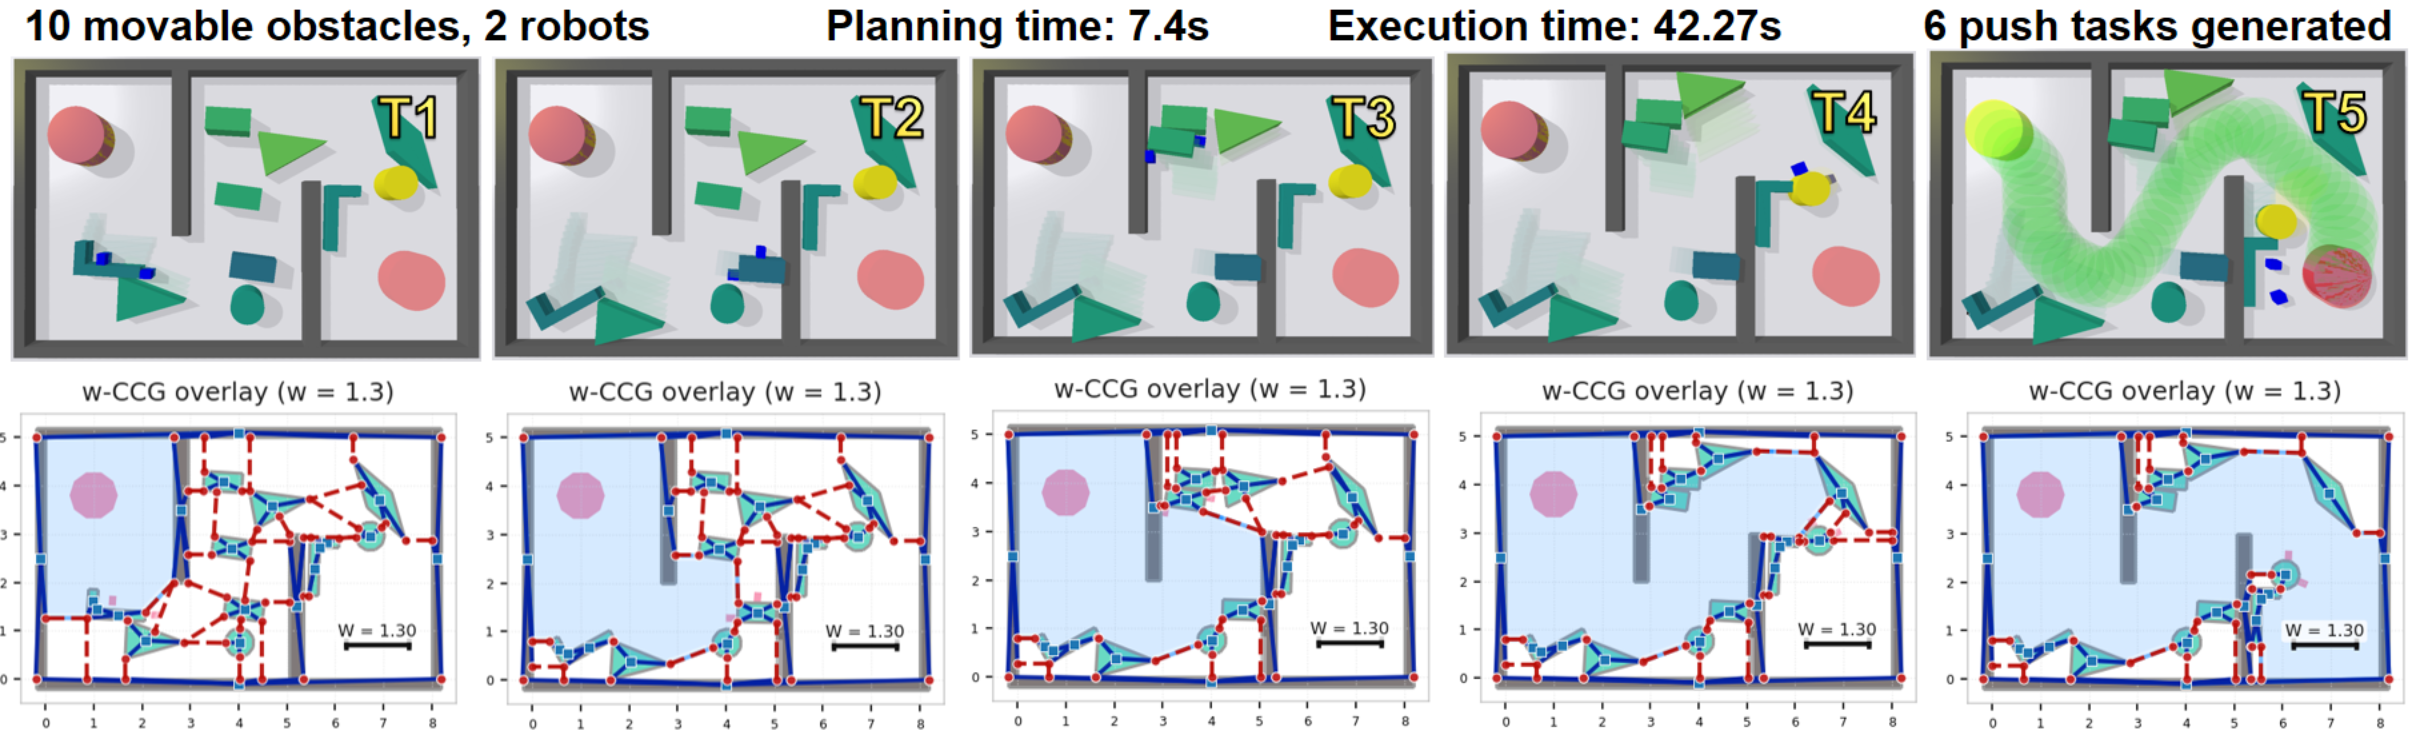
\includegraphics[width=0.95\linewidth]{figures/sim_exp.png}
  \vspace{-0.15in}
\caption{Execution--planning alignment in the main scenario.
\textbf{Top:}~$5$ PyBullet snapshots as~$2$ robots push a cylindrical object.
\textbf{Bottom:} corresponding WCCG overlays with the start face in blue.
The task moves the object from
\(\mathbf{s}^{\texttt{S}}_{\texttt{V}}=(1,4)\) to
\(\mathbf{s}^{\texttt{G}}_{\texttt{V}}=(7,2)\).
In the final state, the start face contains~$G$, matching the executed
trajectory and confirming success.}
\vspace{-0.1in}
\label{fig:simloop}
\end{figure*}
% ========================================

\subsubsection{Termination and Replanning}
Termination occurs when a popped node~$\nu$ reaches a snapshot satisfying the
WCCG clearance certificate in~\eqref{eq:wccg_criterion}. The solution
$\pi^\star$ is obtained by tracing incoming push-task labels to the root and
constitutes a complete solution to~\eqref{eq:problem}. During execution, WCCG,
gap-sequencing cache, and reusable ModeTable entries are updated after each
accepted task. If object drift, transition blockage, or contact loss invalidates
the remaining prefix, the search restarts from the observed snapshot while
preserving failed task signatures and reusable mode entries.

% %%========================================
%==============================
\subsection{Overall Analyses}\label{subsec:overall}

\subsubsection{Execution and Online Adaptation}\label{subsec:execute}
The hybrid search returns a pushing schedule
$\pi = \{\tau_1,\cdots,\tau_K\}$, where
$\tau_k \triangleq (\Omega_k,\mathbf{v}_k,\boldsymbol{\xi}_k)$ specifies
the target obstacle, pushing direction and mode. The schedule is executed
sequentially in a receding-horizon manner. For each $\tau_k$, the robots move
to the required mode~$\boldsymbol{\xi}_k$ for obstacle~$\Omega_k$
and follow the pushing direction~$\mathbf{v}_k$
from the current state as in~\eqref{eq:sim}. On the hardware, optimized contact forces are used for mode feasibility rather than direct force commands; the controller converts the planned contact geometry and object motion into velocity commands with feedback tracking. During transition, robots
are reassigned by preserving the circular order of contact points along the
obstacle boundary~\cite{tang2026pushingbots}, which reduces path crossings
under sufficient clearance. After each push, the system state is updated from
observation, and the execution proceeds to $\tau_{k+1}$ if the action succeeds.
For consistency with execution, the WCCG is rebuilt periodically from
the current configuration. Execution terminates once a $W$-clear path
$\mathcal{P}^W_\texttt{V}$ connects~$\mathbf{x}_\texttt{V}^{\texttt{S}}$ and
$\mathbf{x}_\texttt{V}^{\texttt{G}}$.
Replanning is triggered by observed execution discrepancies, including failed contact establishment, stalled pushing, or invalidated remaining WCCG connectivity. In such cases, Alg.~\ref{alg:pihs} is
called from the current state to derive the updated pushing schedule.

%----------------------------------------------
\subsubsection{Computational Complexity}\label{subsubsec:complexity}

Given~$M$ movable obstacles, the computational cost of one node
expansion in Alg.~\ref{alg:pihs} is dominated by candidate generation and
physics validation. The WCCG update and gap ranking incur
$\mathcal{O}(M\log M+|\mathcal{V}|+|\mathcal{E}_c|+|\mathcal{E}_b|)$ and
$\mathcal{O}(|\Gamma_{\mathcal{L}_\nu}|
\log|\Gamma_{\mathcal{L}_\nu}|)$ costs, respectively, while the dominant
simulation cost is
\[
\mathcal{O}\left(
\sum_{g\in\mathsf{Rank}(\nu)}
|\Xi_g|
\left(
C_{\mathrm{LP}}+
\frac{\rho_\nu T_{\mathrm{sim}}}{n_{\texttt{w}}}
\right)
\right),
\]
Therefore, scalability is mainly determined by validated pushing candidates,
while quick-pass filtering and parallel simulation reduce the practical
expansion cost. Robot-team size mainly affects mode generation, where greedy
contact refinement avoids exhaustive $|\mathcal{A}|^N$ contact assignment and
evaluates bounded single-contact replacements.
%% %----------------------------------------------
%% \subsubsection{Generalization}\label{subsec:general}
%% The framework admits several extensions:
%% (I) \textit{Heterogeneous teams.} Per-robot gain tuning and robot-specific mode
%% priors enable cooperation among diverse robots;
%% (II) \textit{Concurrent pushing.} Multi-object mode generation and conflict-aware
%% transition planning allow multiple obstacles to be pushed simultaneously;
%% (III) \textit{Dynamic environments.} Periodic $W$--connectivity checks and
%% on-demand replanning handle disturbances such as object drift or unmodeled
%% contacts during execution.

% %%========================================
